\documentclass{beamer}
\usepackage{./common_slides}
\usepackage[absolute,overlay]{textpos}
\usepackage{graphicx}


\title{ Distributed Stochastic Gradient Descent }

\author{Kevin Yang and Michael Farrell}
\begin{document}

\begin{frame}w
  \titlepage
\end{frame}

\begin{frame}{Motivation - Deep Learning}

\begin{columns}[T] % align columns
\begin{column}{.48\textwidth}
\begin{itemize}
\item Deep-Learning
\begin{itemize}
\item Objective: Learn a complicated, non-linear function that minimizes some loss function
\end{itemize}
\item Why do we need deep models?
\begin{itemize}
\item The class of linear functions is inadequate for many problems.
\end{itemize}
\end{itemize}
\end{column}%
\hfill%
\begin{column}{.48\textwidth}
\begin{figure}
    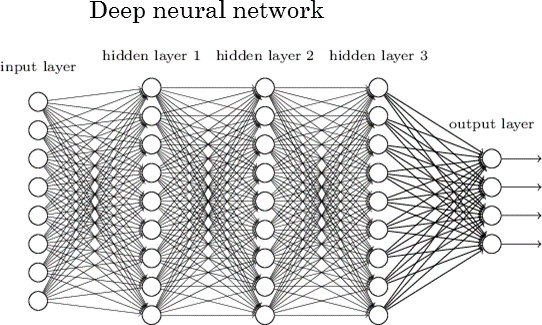
\includegraphics[scale = .35]{./img/deep_learning}
      \caption{\scalebox{.3}{http://www.rsipvision.com/exploring-deep-learning/}}
\end{figure}
\begin{figure}
    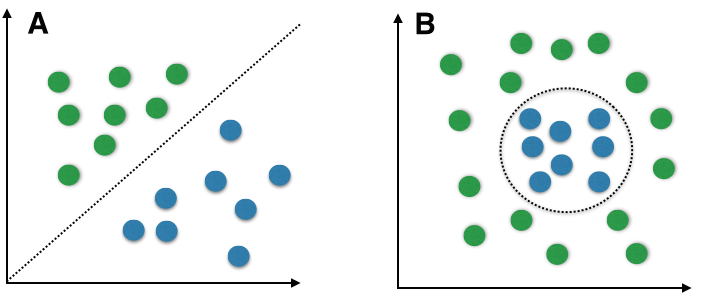
\includegraphics[scale = .17]{./img/lin_v_nonlin}
      \caption{\scalebox{.3}{http://sebastianraschka.com/Articles/2014{\_}naive{\_}bayes{\_}1.html}}
\end{figure}
\end{column}%
\end{columns}
\end{frame}

\begin{frame}{Motivation - Deep Learning}
\begin{itemize}
\item How do we learn these deep models?
\begin{itemize}
\item Choose a random example
\item Run the neural network on the example
\item Adjust the parameters of the network such that our loss function is minimized more than it was before
\item Repeat
\end{itemize}
\pause
\item Difficulties?
\begin{itemize}
\item Local Minima
\item Non-convexity
\item Neural Networks can have millions or even billions of parameters
\end{itemize}
\end{itemize}
\begin{textblock*}{5cm}(8cm,.5cm) % {block width} (coords)
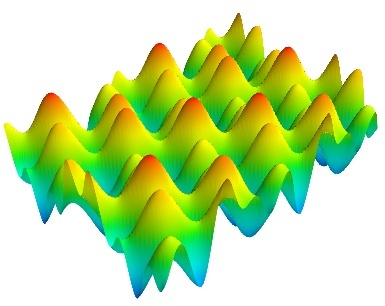
\includegraphics[scale = .3]{./img/2d_func}
\end{textblock*}
\end{frame}

\begin{frame}{Motivation - SGD}
\begin{itemize}
\item How do we maximize our reward function?
\begin{itemize}
\item One common technique is Stochastic Gradient Descent
\item $\mathbf w$ is the vector of parameters for the model
\item $\eta$ is the learning rate 
\item $\mathbf f(\mathbf w)$ is the loss function evaluated with the current parameters $\mathbf w$
\item 
\begin{algorithmic}
\State $\mathbf w \gets \mathbf 0$
\While {$\mathbf f(\mathbf w)$ is not minimized}
	\For {$i = 1, n$}
    \State $\mathbf w \gets \mathbf w - \eta\nabla f(\mathbf w)$
	\EndFor
\EndWhile

\end{algorithmic}
\item As the number of training examples, $n$, and the number of parameters, $|\mathbf w|$, increases, this algorithm quickly becomes very slow...
\end{itemize}
\end{itemize}
\end{frame}

\begin{frame}{Motivation - Distributed SGD}
\begin{itemize}
\item Since some of these models take days/weeks/months to run, we would hope that we could use a distributed computing cluster in order to parallelize this process.
\pause
\item Learn from Google!
\begin{itemize}
\item DistBelief- 2012
\begin{itemize}
\item Downpour SGD
\item Sandblaster L-BFGS
\end{itemize}
\item TensorFlow- 2015
\begin{itemize}
\item gRPC
\end{itemize}
\end{itemize}
\end{itemize}

\end{frame}

\begin{frame}{DistBelief - Downpour SGD}
\begin{itemize}
\item ``An asynchronous stochastic gradient descent procedure supporting a large number of model replicas." \footnote{Diagram taken from Dean et al. \it{Large Scale Distributed Deep Networks}
}
\end{itemize}
$$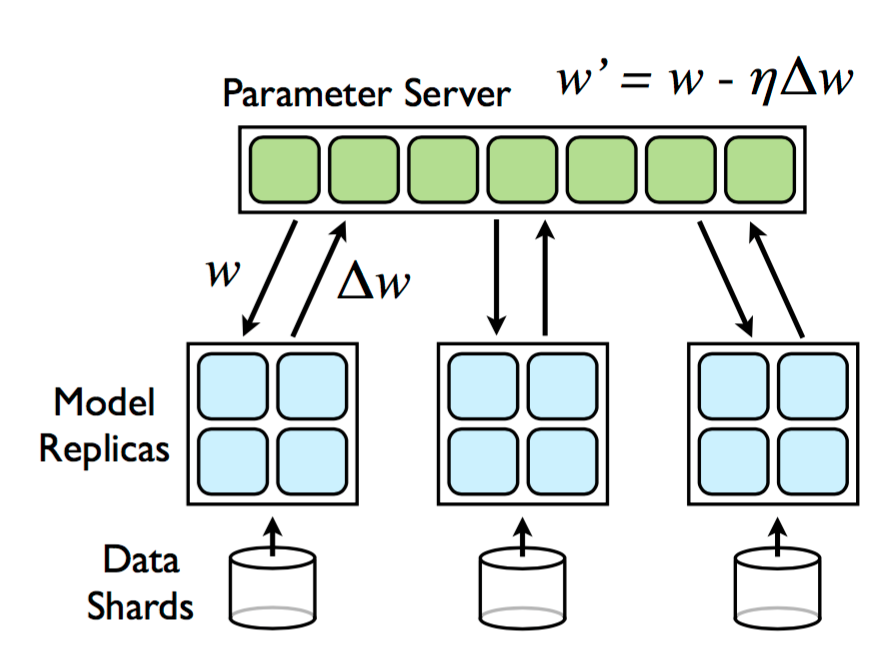
\includegraphics[scale = .5]{./img/downpour}$$
\end{frame}

\begin{frame}{DistBelief - Sandblaster L-BFGS}
\begin{itemize}
\item ``A framework that supports a variety of distributed batch optimization procedures, including a distributed implementation of L-BFGS" \footnote{Diagram taken from Dean et al. \it{Large Scale Distributed Deep Networks}}
\end{itemize}
$$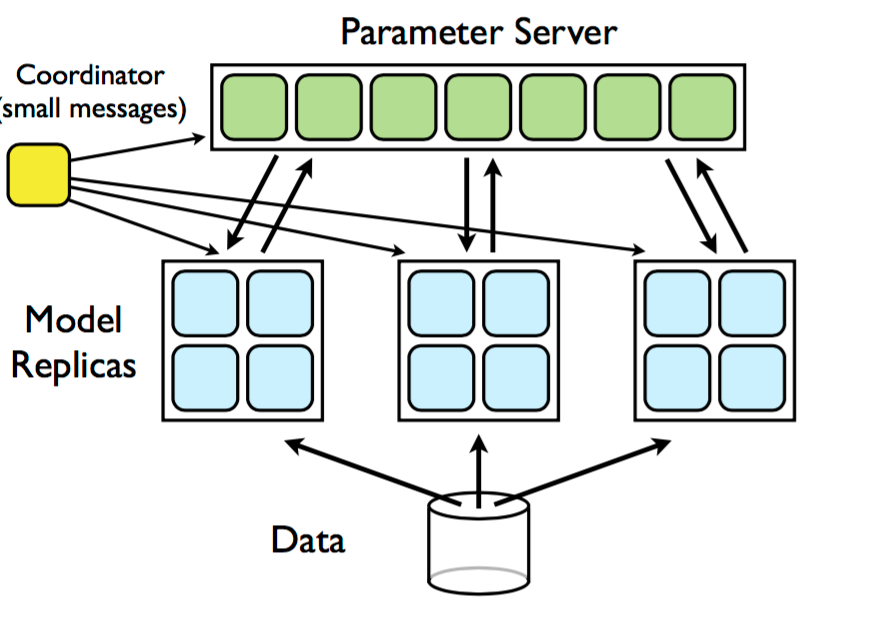
\includegraphics[scale = .5]{./img/sandblaster}$$
\end{frame}

\begin{frame}{TensorFlow-GRPC}
\begin{itemize}
\item Second Generation ML Model focused on distributing models to CPUs and GPUs
\item Uses the high performance RPC framework (GRPC \footnote{Diagram taken from http://www.grpc.io/}) in order to communicate between separate processes 
\begin{itemize}
\item Uses Protocol Buffers -v3
\item C-based
\item Client-server stubs in 10+ languages and counting
\end{itemize}
\end{itemize}
$$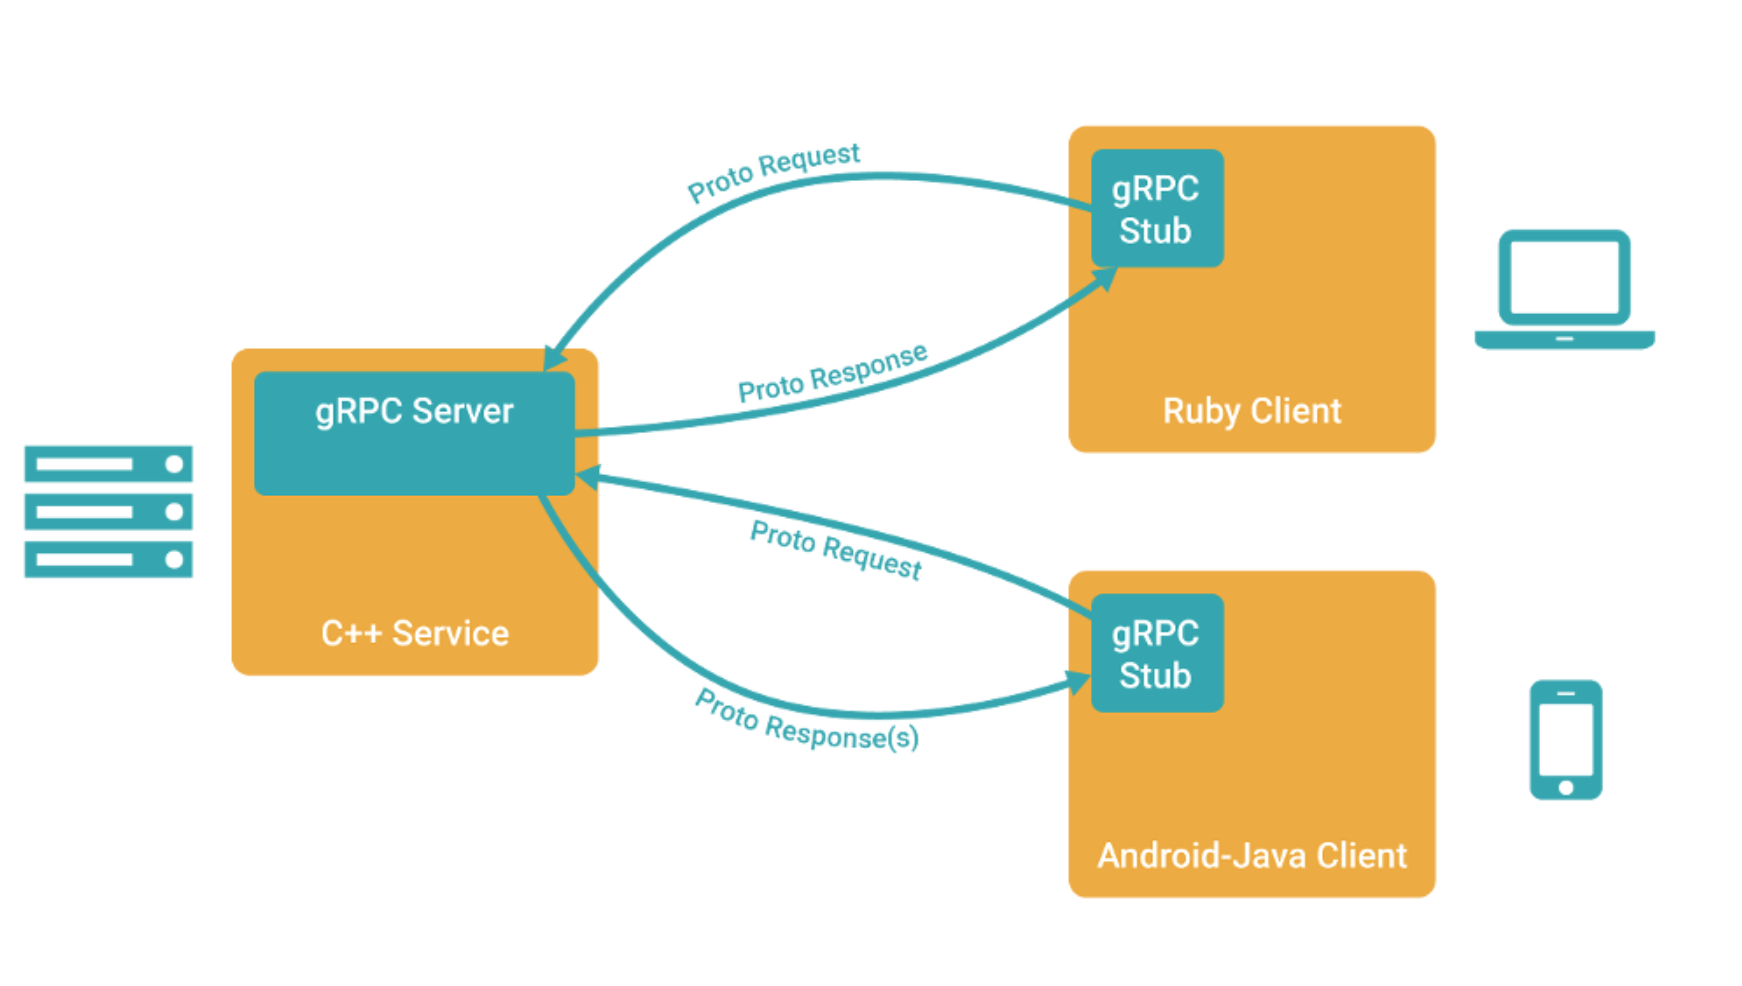
\includegraphics[scale = .2]{./img/gRPC}$$
\end{frame}

\begin{frame}{DistBelief/TensorFlow Summary}
\begin{itemize}
\item TensorFlow is basically the second version of DistBelief that is approximately twice as fast and much more user-friendly.
\item Results from DistBelief" \footnote{Diagram taken from Dean et al. \it{Large Scale Distributed Deep Networks}}:
\end{itemize}
$$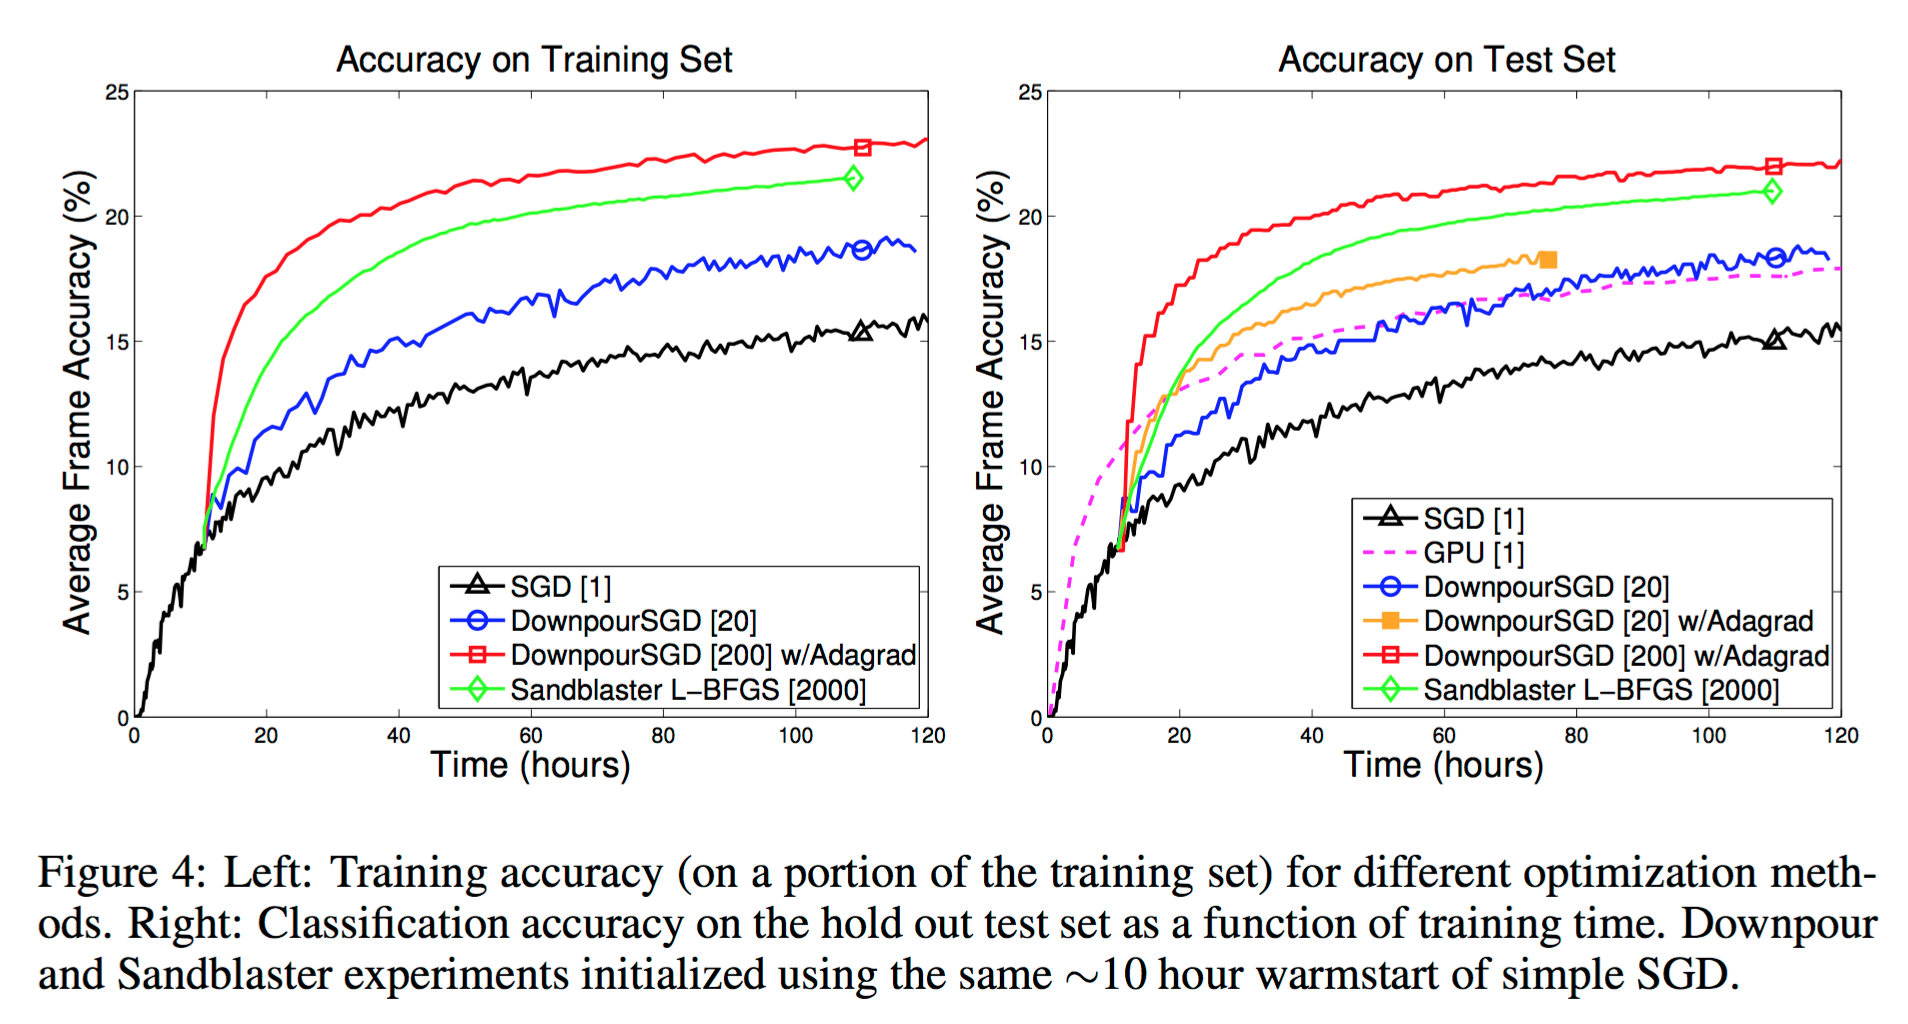
\includegraphics[scale = .18]{./img/dist_train}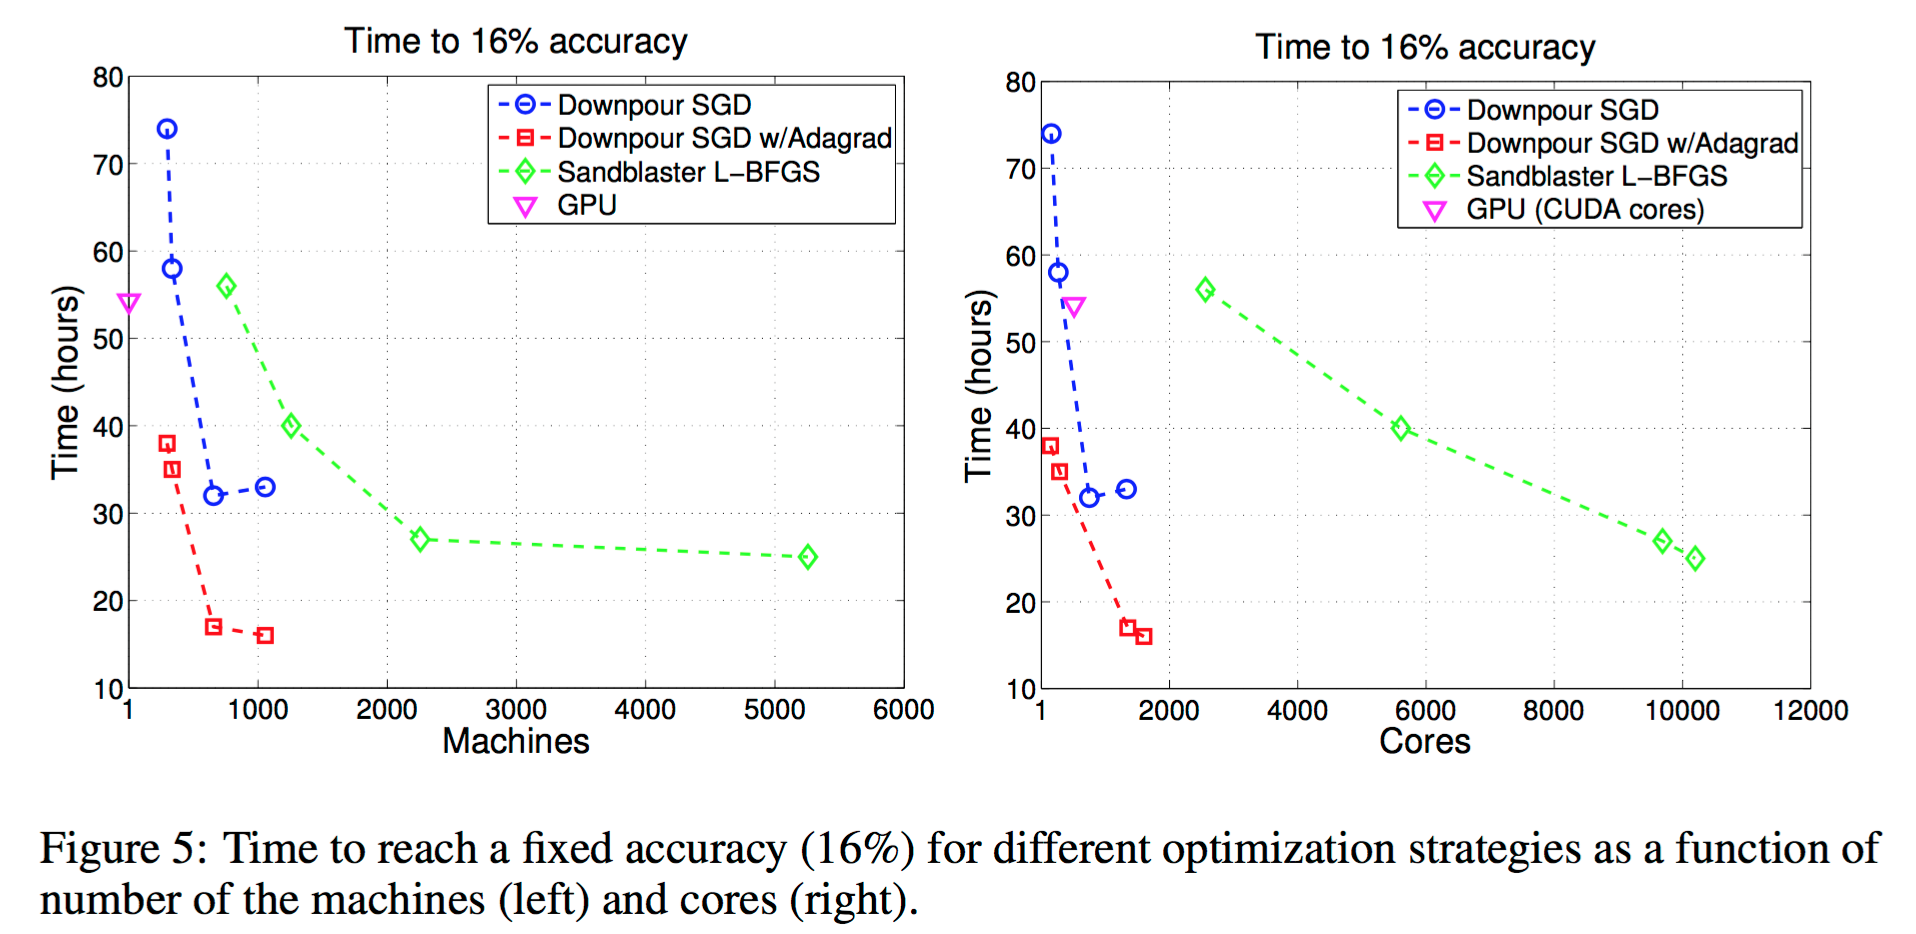
\includegraphics[scale = .18]{./img/dist_16}$$
\end{frame}

\begin{frame}{Our Project}
\begin{itemize}
\item We frequently run into scenarios where we have a model that trains incredibly slowly on our local machines. As a consequence, we hope to benefit from additional cloud computing resources and build our own Distributed SGD system based on DistBelief and TensorFlow systems.
\begin{itemize}
\item The Distributed SGD system will have the user give a function that returns the outputs of a model, a function that returns the gradients of a model, and the number of machines to train the model on.
\item Use GRPC with Protocol Buffers to communicated between processes, similar to TensorFlow.
\item Implement Downpour-SGD which seems to be the most effective model with limited resources.
\end{itemize}
\end{itemize}
\end{frame}


\begin{frame}{Our Example}
\begin{itemize}
\item To test our system, we're working with the Caltech 101 Computational Vision dataset \footnote{L. Fei-Fei, R. Fergus and P. Perona. \it{Learning generative visual models
from few training examples: an incremental Bayesian approach tested on
101 object categories.}}. In this dataset, there are about 20,000 pictures of objects in 101 categories. All of these images are around 300 x 200 pixels in size.
\item We've implemented a convolutional neural net that tries to classify what object is represented in the image.

$$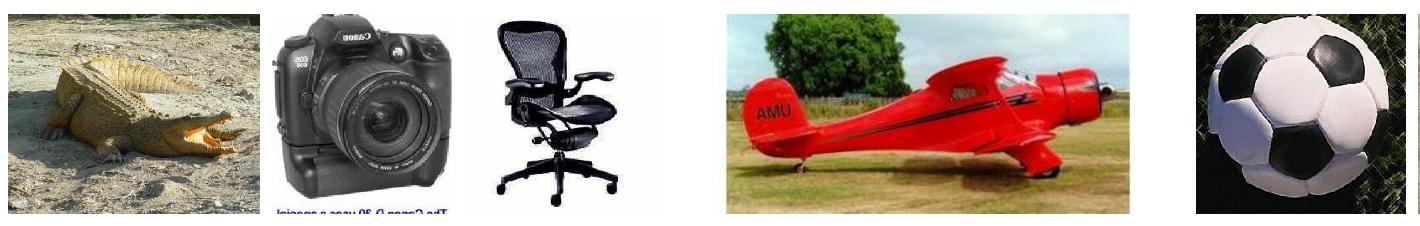
\includegraphics[scale = .30]{./img/dataset.png}$$
\end{itemize}
\end{frame}

\begin{frame}{Computational Resources}
\begin{itemize}
\item We are using Google Cloud Compute Engine to set up VMs and run the code. To run classification on our image dataset, we're using small instances with 6GB of RAM with 2 cores. This has a rate of 7.8 cents per hour.
\item On a machine of this size, running 10 epochs of gradient descent takes 56 minutes.
\item To streamline things, we've preconfigured images of a parameter server and model training server that are already set up with relevant code, tools, and libraries.
\item As a result, setting up and launching the compute instances necessary for model training takes only a couple lines. 
\end{itemize}
\end{frame}

\begin{frame}{Implementing Downpour-SGD}
\begin{itemize}
\item The Downpour-SGD requires the passing of parameters and parameter updates between processes. In our example, we have 74,770,901 parameters and the size of our parameters is 0.5GB.
\item Bottleneck here is the network. Parameters can be $>>$0.5Gb.
\item We can leverage the fact that some of these models are extremely sparse
\begin{itemize}
\item only send parameters updated
\item only update parameters every $n_x$ times
\end{itemize}
\item Explore protocol buffer streams
\end{itemize} 
$$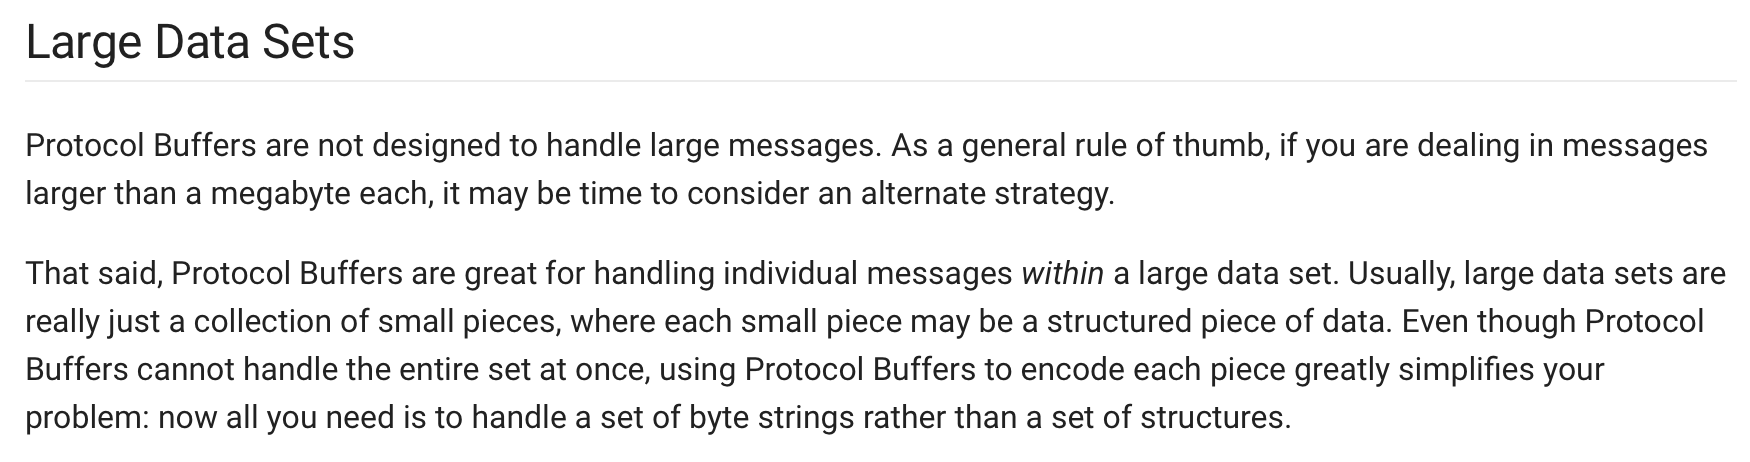
\includegraphics[scale = .27]{./img/large_data}$$
\end{frame}

\begin{frame}{Main Distributed System Challenges}
\begin{itemize}
\item Network Issues
\begin{itemize}
    \item We have to deal with network latency and try to reduce transportation cost as much as possible in order for our models to train properly. 
    \item We would like to experiment with a couple different RPCs to optimize the speed of our system.
\end{itemize}
\item Fault tolerance
\begin{itemize}
    \item We need to make our system as resilient as possible against failures. Because all of these machines are doing a lot of computation while running gradient descent and manipulating parameters, these systems are bound to fail with relatively high frequently.  
    \item Having methods in place to detect and remedy the failure of parameter servers and model replicas will be critical.
\end{itemize}

\end{itemize}
\end{frame}

\end{document}
